
\chapter{O Papel da Informação para a Organização} \label{chapter4}

Neste capítulo, será abordado a importância e a relação entre as tecnologias da informação e comunicação (TICs) e a análise de informações para geração de conhecimentos. Atualmente, o gerenciamento de informações é uma atividade importante a ser desempenhada como forma de auxílio aos processos decisórios e estratégicos no ambiente organizacional. A Seção \ref{41} justifica a necessidade do uso do gerenciamento de informações no ambiente organizacional, além de apresentar os conceitos de dado, informação e conhecimento. A Seção \ref{42} apresenta o conceito de sistema de informação e seus benefícios na gestão de informações, e a Seção \ref{43} lista algumas das características desejáveis para a informação e os principais desafios para o gerenciamento de informações. 

\section{Dado, Informação e Conhecimento} \label{41}

A todo o momento, surge a necessidade do levantamento de novos conhecimentos nos mais diversos setores de atuação, o que justifica a produção e o acúmulo da extensa massa informacional à qual temos acesso. Em vista da crescente produção de dados e informações, pensar em formas de tratamento e organização das mesmas torna-se uma tarefa importante a ser desempenhada pelas organizações. \citet[p. 25-26]{somasundaram2011} afirmam que 
\begin{quotation}
	\textit{" O volume de dados gerenciado pelas empresas as fez criar estratégias de classificação de acordo com o valor dos dados e também regras para gerenciá-los durante o seu ciclo de vida. Essas estratégias trazem vantagens operacionais e reguladoras em nível empresarial e também vantagens gerenciais em nível operacional para a organização."} 
\end{quotation}
	
O gerenciamento de informações surge da necessidade de se organizar e controlar o fluxo de informações produzidas ao decorrer do tempo. Com o advento da Internet e o desenvolvimento das tecnologias atuais, o compartilhamento de informações e conhecimentos se estabelece por meio dos diversos canais de comunicações existentes. \citet{cardoso_machado2008} demonstram a relevância do conhecimento para o ambiente organizacional como facilitador do gerenciamento de ações administrativas e operacionais com maior grau de precisão, inovação, criatividade e flexibilização, o que influi na disponibilização de melhores resultados, sejam estes na forma de produtos ou serviços. 

Na literatura, três conceitos aparecem constantemente na abordagem de gerenciamento de informações: \textit{dado, informação} e \textit{conhecimento}, a serem descritos a seguir. Por vezes, algumas pessoas tendem a associar os termos como sendo sinônimos, embora sejam definições distintas.

 Para \citet{siqueira2005}, dado é a menor unidade, ou unidade primária que compõe a informação. Já \citet{cardoso_machado2008} definem dado como uma forma de representação quantitativa, que por sua vez pode ser guardada e trabalhada em meios computacionais. Para \citet[p. 15]{russo2010}, os dados são \textit{"sinais que não foram processados, correlacionados, integrados, avaliados, ou interpretados de qualquer forma, e, por sua vez, representam matéria-prima a ser utilizada na produção de informações"}.
 
 A informação é o resultado do conjunto de unidades de dados, dotados de significado e relevância para quem a utiliza. Podem assumir diferentes valores, que segundo \citet{siqueira2005}, depende da análise e avaliação humana para ser interpretado. \citet[p. 15 \textit{apud} Lussato (2010)]{russo2010} descreve a informação como \textit{"dados contextualizados, que visam fornecer uma solução para determinada situação de decisão".}
 
 Já o conhecimento pode ser entendido como a soma de informações, ideias, sínteses, reflexões, regras e  avaliações que podem influenciar no modo como direcionamos nossas ações, experiências e decisões, o que envolve um alto grau de abstração humana, visto que cada indivíduo constrói seu próprio conhecimento a partir de vivências e experimentações. \citet[p. 499]{cardoso_machado2008} definem conhecimento como \textit{"inteligência obtida pela experiência".}  O conhecimento, por sua vez, pode ser subdividido em duas categorias: o \textit{explícito}, que é aquele que pode ser codificado e apresentado por meio de uma linguagem formal, sendo mais plausível de ser estruturado, manipulado e transmitido; e o \textit{tácito}, que é o conhecimento abstrato, subjetivo a cada pessoa. Pode ser composto por crenças, valores, perspectivas, vivências e experiências do indivíduo, que são variáveis intangíveis. 
 
 \citet[p. 499 \textit{apud} Carvalho (2000)]{cardoso_machado2008} definem a gestão do conhecimento como \textit{"a área que estuda o modo como as organizações entendem o que elas conhecem, o que elas necessitam conhecer e como elas podem tirar o máximo de proveito do conhecimento"}. Nos últimos anos, as empresas têm percebido cada vez mais o valor do conhecimento para compreender e se adaptar tanto ao ambiente externo quanto o interno da organização, o que resulta em uma maior vantagem competitiva. A prática da gestão do conhecimento possibilita a melhoria do desempenho das atividades administrativas e financeiras da organização, além da formação de capital intelectual. De \citet{wada2012}, é possível observar alguns dos benefícios da gestão do conhecimento, tais como:
\begin{itemize}
	\item sustentabilidade e vantagem competitiva;
	\item melhoria e inovação de produtos e serviços;
	\item aprendizado coletivo e disponibilização de informações;
	\item busca e compartilhamento de capital intelectual (conhecimento);
	\item agilidade e capacidade de resposta aos problemas imediatos;
	\item conscientização da equipe de pessoal sobre os empreendimentos da organização;
	\item estímulo à criatividade e busca por novos conhecimentos.
\end{itemize} 


\section{Sistemas de Informação na Análise de Informações} \label{42}

As TICs estão cada vez mais presentes nos ambientes empresariais, fornecendo recursos e serviços que facilitem a gestão de processos informacionais. Em um ambiente onde o acesso rápido e preciso à informação é necessário, seja para tomada de decisões, consultas ou acompanhamento de atividades, os sistemas de informações agregam velocidade e eficiência ao trabalho de gestão documental e informacional. Há diversas definições para sistemas de informações na literatura. De uma forma geral, um sistema de informação é o conjunto de recursos (que pode incluir pessoas, documentos, equipamentos, ferramentas, computadores e softwares, Internet, entre outros), que formam um todo organizado, com o intuito de se atingir uma determinada atividade-fim ou resultado.

Os sistemas de informação (SI) surgem na perspectiva de facilitar o gerenciamento das informações, e é amplamente utilizado por empresas e corporações que necessitam de métodos gerenciais e administrativos dos valores informacionais produzidos interna ou externamente. \citet{laudon} destaca a influência mútua entre as organizações e os sistemas de informação. É necessário que os sistemas de informação estejam de acordo com o organização, de modo a disponibilizar a informação relevante aos grupos ou setores estratégicos da organização. Por outro lado, a organização deve estar disponível às tendências (adaptações) dos sistemas de informação para se beneficiar de novas tecnologias e transformações.

Em suma,  as atividades realizadas por um sistema de informação envolvem a captura dos dados de entrada, conversão dos dados por meio de etapas de processamento e geração de dados de saída, que são transformados em informações que possam ser interpretadas e avaliadas. Para \citet{laudon}, um sistema de informação realiza atividades de coleta (ou recuperação), processamento, armazenamento e distribuição de informações, com o objetivo de embasar um processo de tomada de decisão. Dentre as vantagens da utilização de um SI, encontram-se a facilidade de gerenciamento, organização e controle dos fluxos de dados, rapidez no acesso e recuperação, integração entre sistemas, além de auxiliar nos processos administrativos, por meio da disponibilização de dados e informações para processos decisórios, gestão estratégica, conhecimento e exploração de novos mercados, estabelecimento de padrões de consumo e criação de novos produtos ou serviços.

Muitos recursos e ferramentas computacionais existentes visam facilitar a gestão de informações. Contudo, cabe à organização fazer uso e realizar um gerenciamento de forma inteligente da massa informacional. Por exemplo, uma empresa de publicidade pode utilizar-se de formulários para conhecer o perfil de seus clientes e potenciais interessados; uma instituição de ensino pode utilizar o histórico dos alunos para um possível acompanhamento escolar; uma empresa de alimentos pode utilizar o relatório de vendas para saber quais produtos são mais vendáveis, entre outros. A Figura \ref{areasTIC} lista algumas das áreas mais beneficiadas pelos recursos de Tecnologia de Informação e Comunicação nos últimos anos. Conforme apontado por \citet[p. 4]{mcgee1994}, \textit{"não é a tecnologia, mas sim o seu uso, que cria valor adicional. O valor da informação depende da informação e do papel desempenhado por ela nas organizações."}  A informação pode assumir um valor diferencial de acordo com quem a produz, quem a utiliza, e para qual fim se destina.
\\
\begin{figure}[!t]
	\centering
	{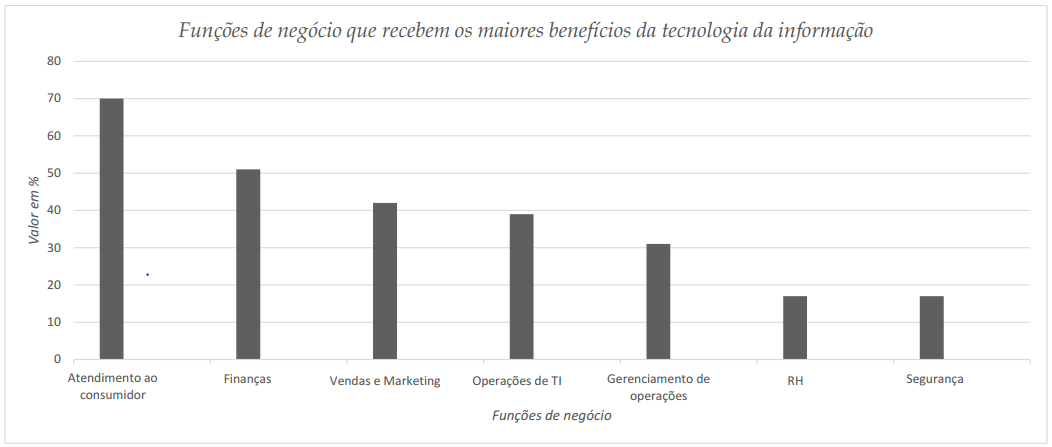
\includegraphics[width=15cm,height=8cm]{images/tic_finalidade}}
	\caption {Áreas mais beneficiadas pelo uso das Tecnologias da Informação~\citep{sistemas_informacao1}.}
	\label{areasTIC}
\end{figure}

\section{Características e Desafios da Informação} \label{43}

\citet{stair2006} listam algumas das características que tornam as informações valiosas para uma organização:
\begin{itemize}
\item \textit{Precisa:} Ausência de erros que podem ser gerados na etapa de processamento de informações imprecisas ou irrelevantes;
\item \textit{Completa:} Presença de todos os detalhamentos essenciais da informação;
\item \textit{Econômica:} O custo de produção deve ser viabilizado pelo valor da informação gerada;
\item \textit{Flexível:} A informação pode ser reutilizada para outros fins além daqueles em que foram aplicados ou utilizados a primeiro momento;
\item \textit{Confiável:} Refere-se a fonte e os processos utilizados para a captura das informações; 
\item \textit{Relevante:} A informação produzida deve fornecer um significado para quem a detém e para o contexto de análise;
\item \textit{Simples:} A informação deve ser objetiva, evitando-se gerar dados que tenham alta complexidade, o que pode comprometer a leitura e interpretação;
\item \textit{Em tempo (pontual):} A informação deve estar disponível e acessível no momento desejado;
\item \textit{Verificável:} A informação deve ser possível de verificação para que se possa atestar a sua validade.  
\end{itemize}

Ao estabelecer uma política de gerenciamento de informações, \citet{somasundaram2011} pontuam os seguintes desafios a serem considerados:

\begin{itemize}
\item \textit{O universo digital em crescimento explosivo:} A quantidade de informações produzidas cresce de modo exponencial. Atividades como duplicação de dados \textit{(backup)} e readaptação de informações contribuem para o aumento massivo de informações;
\item \textit{O aumento na dependência das informações:} Refere-se à necessidade do uso estratégico e inteligente das informações para o alcance dos objetivos da organização, como forma de estabelecer vantagem competitiva e sucesso no mercado;
\item \textit{O valor inconstante das informações:} Trata-se da variabilidade da relevância da informação.  Cada informação produzida pode ter sua durabilidade variada, a depender da relevância da informação para quem a utiliza. O ciclo de vida da informação~\citep{somasundaram2011} determina o valor que informação assume conforme o tempo, com a possibilidade de se agregar maior ou menor importância ao seu conteúdo.
\end{itemize}

\citet[p. 497]{cardoso_machado2008} afirmam que \textit{"a coleta e o armazenamento de dados, por si só, não contribuem para melhorar a estratégia da informação."} Uma análise eficiente dos dados, além de exercer resultados significativos para as atividades existentes, pode contribuir e potencializar o desenvolvimento de atividades e ações futuras. Conforme apontado por \citet[p.288]{laudon}, os sistemas de informação contribuem para gestão do conhecimento, para a melhoria do fluxo de informações e para estabelecer a base de conhecimento das organizações. \textit{"Na medida em que o conhecimento se torna um ativo central, produtivo e estratégico, o sucesso da organização depende cada vez mais da sua habilidade em coletar, produzir, manter e distribuir conhecimento".}


 

	

